\documentclass[aspectratio=169]{beamer}
\usepackage{CustomTheme}

\addbibresource{nlp-for-ch/02-Machine-Translation.bib}

\usepackage{tikzsymbols}

\DeclareTextSymbol{\textstar}{TS1}{136}
\DeclareTextSymbolDefault{\textstar}{TS1}

\newfontfamily{\junicodeFont}{Junicode-Regular.ttf}
\newcommand{\juni}[1]{{\junicodeFont #1}}

\newcommand{\loi}[1]{\textcolor{orange}{#1}}
\newcommand{\red}[1]{\textcolor{red}{\bf #1}}
\newcommand{\ora}[1]{\textcolor{orange}{#1}}
\newcommand{\blue}[1]{\textcolor{blue}{#1}}
\newcommand{\gre}[1]{\textcolor{green}{\bf #1}}
\newcommand{\pink}[1]{\textcolor{pink}{\bf #1}}
\newcommand{\purp}[1]{\textcolor{purple}{\bf #1}}
\newcommand{\mycitation}[1]{\scriptsize{\textcolor{lightgray}{[#1]}}}


\title{Machine translation for ``text tidying''}
\subtitle{A (hidden) key step in computationnal ecdotics}
\author[S. Gabay]{Simon Gabay \inst{1}}
\institute[VFU]{\inst{1} Université de Genève \\ \texttt{simon.gabay@unige.ch}}

\begin{document}

    \begin{frame}
	\titlepage
	\begin{center}
		  CC-BY
	\end{center}
\end{frame}

%---------------------------------------------------------------

    \section{Transcribing}

    \begin{frame}
	\begin{center}
	    Transcribing
	\end{center}
    \end{frame}

%---------------------------------------------------------------

    \begin{frame}{Transcribing}
        \begin{columns}[t]
            \begin{column}{.52\textwidth}
                    \vspace{-1.5em}
                    \begin{figure}
                        \centering
			            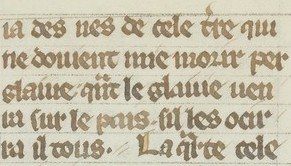
\includegraphics[width=\textwidth,height=0.6\textheight,keepaspectratio]{nlp-for-ch/images/MA_btv1b10465182x_137.jpeg}
                        \caption{\small Abraham Ibn Ezra, \textit{Li livres du commencement de sapience} \tiny{Source: \href{https://gallica.bnf.fr/ark:/12148/btv1b10465182x/f137.item}{Gallica}}}
                        \label{fig:ibnEzra}
                    \end{figure}
                    
                    \vspace{-1em}
                    \textit{ja des nés de cele terre qui ne dovient mie morir per glaive quant le glaive venra sur le païs, s'il les ocirra il tous. La quarte cele}
            \end{column}
            \begin{column}{.48\textwidth}
            \end{column}
        \end{columns}
    \end{frame}

%---------------------------------------------------------------

    \begin{frame}{Transcribing}
        \begin{columns}[t]
            \begin{column}{.52\textwidth}
                    \vspace{-1.5em}
                    \begin{figure}
                        \centering
			            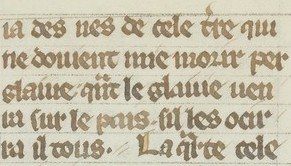
\includegraphics[width=\textwidth,height=0.6\textheight,keepaspectratio]{nlp-for-ch/images/MA_btv1b10465182x_137.jpeg}
                        \caption{\small Abraham Ibn Ezra, \textit{Li livres du commencement de sapience} \tiny{Source: \href{https://gallica.bnf.fr/ark:/12148/btv1b10465182x/f137.item}{Gallica}}}
                        \label{fig:ibnEzra}
                    \end{figure}
                    
                    \vspace{-1em}
                    \textit{ja des nés de cele terre qui ne dovient mie morir per glaive quant le glaive venra sur le païs, s'il les ocirra il tous. La quarte cele}
            \end{column}
            \begin{column}{.48\textwidth}
                \begin{itemize}
                    \item Transcription is an ancient art, which has been thought about extensively for decades (at least) by philologists
                    \item Many problems are known: abbreviations, punctuation, accentuation…
                    \item Over time, terms (semi-diplomatic, diplomatic, etc.) appeared, and practices were (relatively) stabilized.
                \end{itemize}
            \end{column}
        \end{columns}
    \end{frame}

%---------------------------------------------------------------

    \begin{frame}{Towards new practices}
        \begin{columns}[t]
            \begin{column}{.52\textwidth}
                    \vspace{-1.5em}
                    \begin{figure}
                        \centering
			            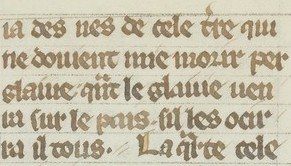
\includegraphics[width=\textwidth,height=0.6\textheight,keepaspectratio]{nlp-for-ch/images/MA_btv1b10465182x_137.jpeg}
                        \caption{\small Abraham Ibn Ezra, \textit{Li livres du commencement de sapience} \tiny{Source: \href{https://gallica.bnf.fr/ark:/12148/btv1b10465182x/f137.item}{Gallica}}}
                        \label{fig:ibnEzra}
                    \end{figure}
                    
                    \vspace{-1em}
                    \textit{ja des nés de cele terre qui ne dovient mie morir per glaive quant le glaive venra sur le païs, s'il les ocirra il tous. La quarte cele}
            \end{column}
            \begin{column}{.48\textwidth}
                \begin{minipage}[t][.48\textheight]{\textwidth}
                    \vspace{.2cm}
                    \red{ı}a \juni{ꝺ}es nes \juni{ꝺ}e cele \juni{t̾}re quı\\ 
                    ne \red{\juni{ꝺ}}ouíent míe mo\juni{ꝛ}ír per\\ 
                    gla\red{í}ue q\juni{nͣ}t le glaíue uen\\ 
                    ra \red{\juni{ſ}}ur le paıs. \juni{ſ}ıl les ocír\\ 
                    ra il tous. La \red{\juni{qͣ}}rte cele
                \end{minipage}\par
                \begin{minipage}[t][.48\textheight]{\textwidth}
             
                \end{minipage}
            \end{column}
        \end{columns}
    \end{frame}

%---------------------------------------------------------------

    \begin{frame}{Towards new practices}
        \small
        \begin{columns}[t]
            \begin{column}{.52\textwidth}
                    \vspace{-1.5em}
                    \begin{figure}
                        \centering
			            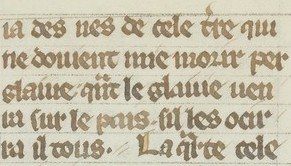
\includegraphics[width=\textwidth,height=0.6\textheight,keepaspectratio]{nlp-for-ch/images/MA_btv1b10465182x_137.jpeg}
                        \caption{\small Abraham Ibn Ezra, \textit{Li livres du commencement de sapience} \tiny{Source: \href{https://gallica.bnf.fr/ark:/12148/btv1b10465182x/f137.item}{Gallica}}}
                        \label{fig:ibnEzra}
                    \end{figure}
                    
                    \vspace{-1em}
                    \textit{ja des nés de cele terre qui ne dovient mie morir per glaive quant le glaive venra sur le païs, s'il les ocirra il tous. La quarte cele}
            \end{column}
            \begin{column}{.48\textwidth}
                \begin{minipage}[t][.48\textheight]{\textwidth}
                    \vspace{.2cm}
                    \juni{\red{ı}a \juni{ꝺ}es nes \juni{ꝺ}e cele \juni{t̾}re quı\\ 
                    ne \red{\juni{ꝺ}}ouíen\juni{ꞇ} míe mo\juni{ꝛ}ír per\\ 
                    gla\red{í}ue q\juni{nͣ}\juni{ꞇ} le glaíue uen\\ 
                    ra \red{\juni{ſ}}ur le paıs. \juni{ſ}ıl les ocír\\ 
                    ra il \juni{ꞇ}ous. La \red{\juni{qͣ}}r\juni{ꞇ}e cele}
                \end{minipage}\par
                \begin{minipage}[t][.48\textheight]{\textwidth}
                    With the advent of computational philology, these two tasks have become clearly separated:
                    \begin{itemize}
                        \item Transcribing the text.
                        \item Tydying up the text.
                    \end{itemize}               
                \end{minipage}
            \end{column}
        \end{columns}
    \end{frame}

%---------------------------------------------------------------

    \section{Normalising}

    \begin{frame}
	\begin{center}
	    Normalising
	\end{center}
    \end{frame}

%---------------------------------------------------------------

    \begin{frame}[t]{A case study}
        \vspace{1em}
        \begin{table}[htp]
            \centering
            \resizebox{.8\linewidth}{!}{
            \begin{tabular}{l|l}
        	Aquella noche el viejo \red{R}ey de Atenas, & 
                Aquella noche el viejo \gre{r}ey de Atenas \\
        	Concertadas de\red{xò} las triſtes bodas, & 
                concertadas de\gre{jó} las tristes bodas, \\
        	De ag\red{u}eros ciertos, y de enojos llenas, &
                de ag\gre{ü}eros ciertos y de enojos llenas, \\
        	Puesto que alegres y engañadas todas. &
                puesto que alegres y engañadas todas; \\
        	\red{Porque} dulce principio amor ordenas, &
                \gre{¿por qué} dulce principio, Amor, ordenas, \\
        	Donde tr\red{a}gicos fines acomodas? &
                donde tr\gre{á}gicos fines acomodas? \\
        	Aì dieras ocaſion contra ſu efeto, &
                \gre{¡}ay\gre{!} Dieras ocasión contra su efeto, \\
        	\red{Sino} te e\red{ſ}cusa el celeſtial decreto. &
                \gre{si no} te e\gre{x}cusa el celestial decreto.
            \end{tabular}
            }
            \caption{Lope de Vega, \textit{La Filomena}: 1621 version vs 2004 edition.}
            \label{tab:lope}
        \end{table}
        \vspace{-2em}
    \end{frame}

%---------------------------------------------------------------

    \begin{frame}[t]{A case study}
        \vspace{1em}
        \begin{table}[htp]
            \centering
            \resizebox{.8\linewidth}{!}{
            \begin{tabular}{l|l}
        	Aquella noche el viejo Rey de Atenas, & 
                Aquella noche el viejo rey de Atenas \\
        	Concertadas dexò las triſtes bodas, & 
                concertadas dejó las tristes bodas, \\
        	De agueros ciertos, y de enojos llenas, &
                de agüeros ciertos y de enojos llenas, \\
        	Puesto que alegres y engañadas todas\red{.} &
                puesto que alegres y engañadas todas\red{;} \\
        	Porque dulce principio amor ordenas, &
                \red{¿}por qué dulce principio\red{,} Amor\red{,} ordenas, \\
        	Donde tragicos fines acomodas? &
                donde trágicos fines acomodas? \\
        	Aì dieras ocaſion contra ſu efeto, &
                \red{¡}ay\red{!} Dieras ocasión contra su efeto, \\
        	Sino te eſcusa el celeſtial decreto. &
                si no te excusa el celestial decreto.
            \end{tabular}
            }
            \caption{Lope de Vega, \textit{La Filomena}: 1621 version vs 2004 edition.}
            \label{tab:punctuation}
        \end{table}
        \vspace{-2em}
        \begin{itemize}
            \small
                \item \red{Punctuation}
            \end{itemize}
    \end{frame}

%---------------------------------------------------------------

    \begin{frame}[t]{A case study}
        \vspace{1em}
        \begin{table}[htp]
            \centering
            \resizebox{.8\linewidth}{!}{
            \begin{tabular}{l|l}
        	Aquella noche el viejo Rey de Atenas, & 
                Aquella noche el viejo rey de Atenas \\
        	Concertadas dexò las tri\gre{ſ}tes bodas, & 
                concertadas dejó las tri\gre{s}tes bodas, \\
        	De agueros ciertos, y de enojos llenas, &
                de agüeros ciertos y de enojos llenas, \\
        	Puesto que alegres y engañadas todas\red{.} &
                puesto que alegres y engañadas todas\red{;} \\
        	Porque dulce principio amor ordenas, &
                \red{¿}por qué dulce principio\red{,} Amor\red{,} ordenas, \\
        	Donde tragicos fines acomodas? &
                donde trágicos fines acomodas? \\
        	Aì dieras oca\gre{ſ}ion contra \gre{ſ}u efeto, &
                \red{¡}ay\red{!} Dieras oca\gre{s}ión contra \gre{s}u efeto, \\
        	Sino te eſcusa el cele\gre{ſ}tial decreto. &
                si no te excusa el cele\gre{s}tial decreto.
            \end{tabular}
            }
            \caption{Lope de Vega, \textit{La Filomena}: 1621 version vs 2004 edition.}
            \label{tab:allographs}
        \end{table}
        \vspace{-2em}
        \begin{itemize}
            \small
            \item \red{Punctuation}
            \item \gre{Allographs}
        \end{itemize}
    \end{frame}

%---------------------------------------------------------------

    \begin{frame}[t]{A case study}
        \vspace{1em}
        \begin{table}[htp]
            \centering
            \resizebox{.8\linewidth}{!}{
            \begin{tabular}{l|l}
        	Aquella noche el viejo \blue{R}ey de Atenas, & 
                Aquella noche el viejo \blue{r}ey de Atenas \\
        	Concertadas dexò las tri\gre{ſ}tes bodas, & 
                concertadas dejó las tri\gre{s}tes bodas, \\
        	De agueros ciertos, y de enojos llenas, &
                de agüeros ciertos y de enojos llenas, \\
        	Puesto que alegres y engañadas todas\red{.} &
                puesto que alegres y engañadas todas\red{;} \\
        	Porque dulce principio \blue{a}mor ordenas, &
                \red{¿}por qué dulce principio\red{,} \blue{A}mor\red{,} ordenas, \\
        	Donde tragicos fines acomodas? &
                donde trágicos fines acomodas? \\
        	Aì dieras oca\gre{ſ}ion contra \gre{ſ}u efeto, &
                \red{¡}ay\red{!} Dieras oca\gre{s}ión contra \gre{s}u efeto, \\
        	Sino te eſcusa el cele\gre{ſ}tial decreto. &
                si no te excusa el cele\gre{s}tial decreto.
            \end{tabular}
            }
            \caption{Lope de Vega, \textit{La Filomena}: 1621 version vs 2004 edition.}
            \label{tab:capital}
        \end{table}
        \vspace{-2em}
        \begin{itemize}
            \small
            \item \red{Punctuation}
            \item \gre{Allographs}
            \item \blue{Capital letters}
        \end{itemize}
    \end{frame}

%---------------------------------------------------------------

    \begin{frame}[t]{A case study}
        \vspace{1em}
        \begin{table}[htp]
            \centering
            \resizebox{.8\linewidth}{!}{
            \begin{tabular}{l|l}
        	Aquella noche el viejo \blue{R}ey de Atenas, & 
                Aquella noche el viejo \blue{r}ey de Atenas \\
        	Concertadas de\ora{x}ò las tri\gre{ſ}tes bodas, & 
                concertadas de\ora{j}ó las tri\gre{s}tes bodas, \\
        	De agueros ciertos, y de enojos llenas, &
                de agüeros ciertos y de enojos llenas, \\
        	Puesto que alegres y engañadas todas\red{.} &
                puesto que alegres y engañadas todas\red{;} \\
        	Porque dulce principio \blue{a}mor ordenas, &
                \red{¿}por qué dulce principio\red{,} \blue{A}mor\red{,} ordenas, \\
        	Donde tragicos fines acomodas? &
                donde trágicos fines acomodas? \\
        	Aì dieras oca\gre{ſ}ion contra \gre{ſ}u efeto, &
                \red{¡}ay\red{!} Dieras oca\gre{s}ión contra \gre{s}u efeto, \\
        	Sino te e\ora{ſ}cusa el cele\gre{ſ}tial decreto. &
                si no te e\ora{x}cusa el cele\gre{s}tial decreto.
            \end{tabular}
            }
            \caption{Lope de Vega, \textit{La Filomena}: 1621 version vs 2004 edition.}
            \label{tab:spelling}
        \end{table}
        \vspace{-2em}
        \begin{itemize}
            \small
            \item \red{Punctuation}
            \item \gre{Allographs}
            \item \blue{Capital letters}
            \item \ora{Spelling} (if it does not affect the pronunciation)
        \end{itemize}
    \end{frame}

%---------------------------------------------------------------

    \begin{frame}[t]{A case study}
        \vspace{1em}
        \begin{table}[htp]
            \centering
            \resizebox{.8\linewidth}{!}{
            \begin{tabular}{l|l}
        	Aquella noche el viejo \blue{R}ey de Atenas, & 
                Aquella noche el viejo \blue{r}ey de Atenas \\
        	Concertadas de\ora{x}\pink{ò} las tri\gre{ſ}tes bodas, & 
                concertadas de\ora{j}\pink{ó} las tri\gre{s}tes bodas, \\
        	De ag\pink{u}eros ciertos, y de enojos llenas, &
                de ag\pink{ü}eros ciertos y de enojos llenas, \\
        	Puesto que alegres y engañadas todas\red{.} &
                puesto que alegres y engañadas todas\red{;} \\
        	Porque dulce principio \blue{a}mor ordenas, &
                \red{¿}por qué dulce principio\red{,} \blue{A}mor\red{,} ordenas, \\
        	Donde tr\pink{a}gicos fines acomodas? &
                donde tr\pink{á}gicos fines acomodas? \\
        	Aì dieras oca\gre{ſ}i\pink{o}n contra \gre{ſ}u efeto, &
                \red{¡}ay\red{!} Dieras oca\gre{s}i\pink{ó}n contra \gre{s}u efeto, \\
        	Sino te e\ora{ſ}cusa el cele\gre{ſ}tial decreto. &
                si no te e\ora{x}cusa el cele\gre{s}tial decreto.
            \end{tabular}
            }
            \caption{Lope de Vega, \textit{La Filomena}: 1621 version vs 2004 edition.}
            \label{tab:accents}
        \end{table}
        \vspace{-2em}
        \begin{itemize}
            \small
            \item \red{Punctuation}
            \item \gre{Allographs}
            \item \blue{Capital letters}
            \item \ora{Spelling} (if it does not affect the pronunciation)
            \item \pink{Accents}
        \end{itemize}
    \end{frame}

%---------------------------------------------------------------

    \begin{frame}[t]{A case study}
        \vspace{1em}
        \begin{table}[htp]
            \centering
            \resizebox{.8\linewidth}{!}{
            \begin{tabular}{l|l}
        	Aquella noche el viejo \blue{R}ey de Atenas, & 
                Aquella noche el viejo \blue{r}ey de Atenas \\
        	Concertadas de\ora{x}\pink{ò} las tri\gre{ſ}tes bodas, & 
                concertadas de\ora{j}\pink{ó} las tri\gre{s}tes bodas, \\
        	De ag\pink{u}eros ciertos, y de enojos llenas, &
                de ag\pink{ü}eros ciertos y de enojos llenas, \\
        	Puesto que alegres y engañadas todas\red{.} &
                puesto que alegres y engañadas todas\red{;} \\
        	\purp{Porque} dulce principio \blue{a}mor ordenas, &
                \red{¿}\purp{por qué} dulce principio\red{,} \blue{A}mor\red{,} ordenas, \\
        	Donde tr\pink{a}gicos fines acomodas? &
                donde tr\pink{á}gicos fines acomodas? \\
        	Aì dieras oca\gre{ſ}i\pink{o}n contra \gre{ſ}u efeto, &
                \red{¡}ay\red{!} Dieras oca\gre{s}i\pink{ó}n contra \gre{s}u efeto, \\
        	\purp{Sino} te e\ora{ſ}cusa el cele\gre{ſ}tial decreto. &
                \purp{si no} te e\ora{x}cusa el cele\gre{s}tial decreto.
            \end{tabular}
            }
            \caption{Lope de Vega, \textit{La Filomena}: 1621 version vs 2004 edition.}
            \label{tab:segmentation}
        \end{table}
        \vspace{-2em}
        \begin{itemize}
            \small
            \item \red{Punctuation}
            \item \gre{Allographs}
            \item \blue{Capital letters}
            \item \ora{Spelling} (if it does not affect the pronunciation)
            \item \pink{Accents}
            \item \purp{Segmentation}
        \end{itemize}
    \end{frame}

%---------------------------------------------------------------

    \begin{frame}[t]{A case study}
        \vspace{1em}
        \begin{table}[htp]
            \centering
            \resizebox{.8\linewidth}{!}{
            \begin{tabular}{l|l}
        	Aquella noche el viejo \blue{R}ey de Atenas, & 
                Aquella noche el viejo \blue{r}ey de Atenas \\
        	Concertadas de\ora{x}\pink{ò} las tri\gre{ſ}tes bodas, & 
                concertadas de\ora{j}\pink{ó} las tri\gre{s}tes bodas, \\
        	De ag\pink{u}eros ciertos, y de enojos llenas, &
                de ag\pink{ü}eros ciertos y de enojos llenas, \\
        	Puesto que alegres y engañadas todas\red{.} &
                puesto que alegres y engañadas todas\red{;} \\
        	\purp{Porque} dulce principio \blue{a}mor ordenas, &
                \red{¿}\purp{por qué} dulce principio\red{,} \blue{A}mor\red{,} ordenas, \\
        	Donde tr\pink{a}gicos fines acomodas? &
                donde tr\pink{á}gicos fines acomodas? \\
        	Aì dieras oca\gre{ſ}i\pink{o}n contra \gre{ſ}u efeto, &
                \red{¡}ay\red{!} Dieras oca\gre{s}i\pink{ó}n contra \gre{s}u efeto, \\
        	\purp{Sino} te e\ora{ſ}cusa el cele\gre{ſ}tial decreto. &
                \purp{si no} te e\ora{x}cusa el cele\gre{s}tial decreto.
            \end{tabular}
            }
            \caption{Lope de Vega, \textit{La Filomena}: 1621 version vs 2004 edition.}
        \end{table}
        \vspace{-1em}
        In this example, some tasks:
        \begin{itemize}
            \item are trivial: \gre{allographs}, \pink{accents}, \ora{spelling};
            \item are not trivial: \purp{segmentation}, \red{punctuation}, \blue{capital letters}.
        \end{itemize}
    \end{frame}

%---------------------------------------------------------------


    \begin{frame}{Using rules?}
        In computationnal words, certain changes:
        \begin{itemize}
            \item can be addressed with rules, such as \textit{ſ} $\to$ \textit{s}
            \item cannot be addressed with (simple) rules:
            \begin{itemize}
                \item \textit{sino} $\to$ \textit{sino} (\textit{No es cantante, sino actor}, ``He is not a singer, but an actor'');
                \item \textit{sino} $\to$ \textit{si no} (\textit{Si no llueve, iremos a la playa.}, ``If it doesn’t rain, we’ll go to the beach.'').
            \end{itemize}
        \end{itemize}
    \end{frame}



%---------------------------------------------------------------

    \section{Machine translation}

    \begin{frame}
	\begin{center}
	    Machine translation
	\end{center}
    \end{frame}

%---------------------------------------------------------------

    \begin{frame}{Machine translation}
        \begin{columns}[t]
            \begin{column}{.48\textwidth}
                \begin{minipage}[t][.42\textheight]{\textwidth}
                    Machine Translation (MT) is use of computational techniques to translate text or speech from one language to another, including the contextual, idiomatic and pragmatic nuances of both languages.
                \end{minipage}
                \begin{minipage}[t][.42\textheight]{\textwidth}
                    \textit{
                    La traduzione automatica è l'uso di tecniche computazionali per tradurre un testo o un discorso da una lingua all'altra, comprese le sfumature contestuali, idiomatiche e pragmatiche di entrambe le lingue.}
                \end{minipage}
            \end{column}
            \begin{column}{.48\textwidth}
                \begin{minipage}[t][.42\textheight]{\textwidth}

                \end{minipage}\par
                \begin{minipage}[t][.42\textheight]{\textwidth}
             
                \end{minipage}
            \end{column}
        \end{columns}
    \end{frame}


%---------------------------------------------------------------

    \begin{frame}{Machine translation}
        \begin{columns}[t]
            \begin{column}{.48\textwidth}
                \begin{minipage}[t][.42\textheight]{\textwidth}
                    Machine Translation (MT) is use of computational techniques to translate text or speech from one language to another, including the contextual, idiomatic and pragmatic nuances of both languages.
                \end{minipage}
                \begin{minipage}[t][.42\textheight]{\textwidth}
                    \hspace{0pt}
                    \centering
                    \vfill
                    English $\to$ Italian
                    \vfill
                    \hspace{0pt}
                \end{minipage}
            \end{column}
            \begin{column}{.48\textwidth}
                \begin{minipage}[t][.42\textheight]{\textwidth}
                    Rather than translating text or speech from one language to another, could we not ``translate'' from one historical state of the language to another?
                \end{minipage}\par
                \begin{minipage}[t][.42\textheight]{\textwidth}
                    \hspace{0pt}
                    \centering
                    \vfill
                    OCR output $\to$ Edited text
                    \vfill
                    \hspace{0pt}
                \end{minipage}
            \end{column}
        \end{columns}
    \end{frame}

%---------------------------------------------------------------

    \begin{frame}{An efficient solution}
        MT can handle complex cases such as translation in cases other than one-to-one translation.
        \begin{table}[]
            \centering
            \begin{tabular}{c||ccccccc}
                English & I & 'm & going & to & the & restaurant & . \\
                Italian & \multicolumn{3}{c}{Vado} & \multicolumn{2}{c}{al} & ristorante & . \\
            \end{tabular}
            \label{tab:problems}
        \end{table}

        Machine translation is already used for tasks other than 'translation' in the strict sense, such as the linguistic normalization of text messages:

	   \begin{table}[h]
	       \centering
	       \begin{tabular}{ccccccc}
	       G & repris & vendredi  & ms & wè & c & cool  \\
	       J'ai & repris & vendredi & mais & ouais & c'est & cool
	       \end{tabular}
	      % \caption{Normalisation (tweets, SMS\dots)}
	       \label{tab:normalisation}
	    \end{table}
    \end{frame}

%---------------------------------------------------------------

    \begin{frame}{Training}

        To train a normalization model, the groundtruth contains a source version and a version of the same text.
        
        \begin{table}\tiny
            \begin{tabular}{l|l}
                \toprule
                \textbf{Source} & \textbf{Target}\\
                \midrule
        	And chiefly thou, O Spirit, that dost prefer &
                And chiefly you, O spirit, that do prefer\\
        	Before all temples th' upright heart and pure &
                Before all temples the upright heart and pure \\
        	Instruct me, for thou know'st, thou from the first &
                Instruct me, for you know, you from the first \\
        	Wast present and with mighty wings outspread &
                Were present, and with mighty wings outspread \\
        	Dove-like sat'st brooding on the vast abyss &
                Dove-like sat brooding on the vast abyss  \\
        	And mad'st it pregnant. What in me is dark & 
                And made it pregnant. What in me is dark \\
        	Illumine, what is low raise and support, &
                Illumine, what is low raise and support,\\
        	That to the heighth of this great argument &
                That to the height of this great argument\\
        	I may assert Eternal Providence &
                I may assert Eternal Providence \\
        	And justify the ways of God to men. &
                And justify the ways of God to men \\
                \bottomrule
            \end{tabular}
            \caption{Milton's \textit{Paradise Lost}.}
        \label{tab:milton}
        \end{table}

        Rather than teaching the machine rules, we will ask it to deduce rules from examples.
        
    \end{frame}

%---------------------------------------------------------------

    \begin{frame}{Methods}
    
        Machine translation can be achieved using a variety of computer methods (presented here in the order in which they appeared):
        
        \begin{itemize}
            \item Rule-based Machine Translation (RBMT), which requires explicit description of each and every linguistic rule;
            \item Statistical Machine Translation (SMT) tries to find patterns and rules in a parallel corpus;
            \item Neural Machine Translation (NMT) is a data-driven method that uses neural networks to model the relationship between the source and the target through a neural network. It can be done with several architectures:
                \begin{itemize}
                    \item LSTM;
                    \item Transformers;
                    \item …
                \end{itemize}
        \end{itemize}
        
    \end{frame}

%---------------------------------------------------------------

    \begin{frame}{Granularity}
        To train a model, several levels are considered
        \begin{itemize}
            \item word level: the sentence is kept as it is after preprocessing (e.g. tokenization);
            \item subword level, or Byte Pair Encoding (BPE) -- \texttt{@@} after a subword unit specifies that the unit does not terminate the word;
            \item character level -- the space is replaced by \textstar\ .
        \end{itemize}
        
        \begin{table}[!h]
	        \centering \scriptsize %
            \begin{tabular}{c|ll}
            Granularity        & Version &  Sentence \\
            \hline
            Word          & Source & Cherchons avec empreſſement \\
                         & Target  & Cherchons avec empressement \\
            BPE          & Source & Ch@@ er@@ ch@@ ons avec em@@ preſ@@ ſement \\
                         & Target  & Ch@@ er@@ ch@@ ons avec em@@ pr@@ ess@@ ement \\
            Character   & Source & C h e r c h o n s \textstar\ a v e c \textstar\ e m p r e ſ ſ e m e n t \\
                        & Target  & C h e r c h o n s \textstar\ a v e c \textstar\ e m p r e s s e m e n t 
            \end{tabular}
        \end{table}

    \end{frame}

%---------------------------------------------------------------
    \begin{frame}{Dangers}
        \vspace{.5em}
        Neural networks are extremely efficient, but they can lead to what are called ``hallucinations''.

        \begin{table}[!h]
            \centering \scriptsize
            \begin{tabular}{p{1.2cm}|p{8cm}} 
            \toprule
            Status & Text \\
            \midrule
            Source   & En cet eſtat \textbf{la}, Monſeigneur, il n'y a point d'apparence de ſonger à la Valtoline, ny de ietter les yeux ſur le bien d'autruy cependant qu'on nous \textbf{diſpute} le \textbf{noſtre}, \& qu'il faut que nous le \textbf{tenions} auecque les deux mains de peur qu'il ne nous \textbf{eſchappe}.\\
            \midrule
            Prediction   & En cet état \gre{là}, Monseigneur, il n'y a point d'apparence de songer à la Valteline, ni de jeter les yeux sur le bien d'autrui cependant qu'on nous \gre{dispute} le \gre{nôtre}, et qu'il faut que nous le \red{commun} avec les deux mains de peur qu'il ne nous \red{apportée}.\\
            \bottomrule
            \end{tabular}
            \caption{Examples of hallucinations with neural-MT.}
        \end{table}
        
        Hallucinations are responses generated by AI that contains false or misleading informations presented as fact.
        
    \end{frame}

%---------------------------------------------------------------

    \begin{frame}{Over- vs under-modifications of the source}
        \vspace{1em}
        To avoid problems, we can use safer approaches, which tend however to ``forget'' some cases.
        
        \begin{columns}
            \begin{column}{.48\textwidth}
                \begin{figure}
                    \centering
                    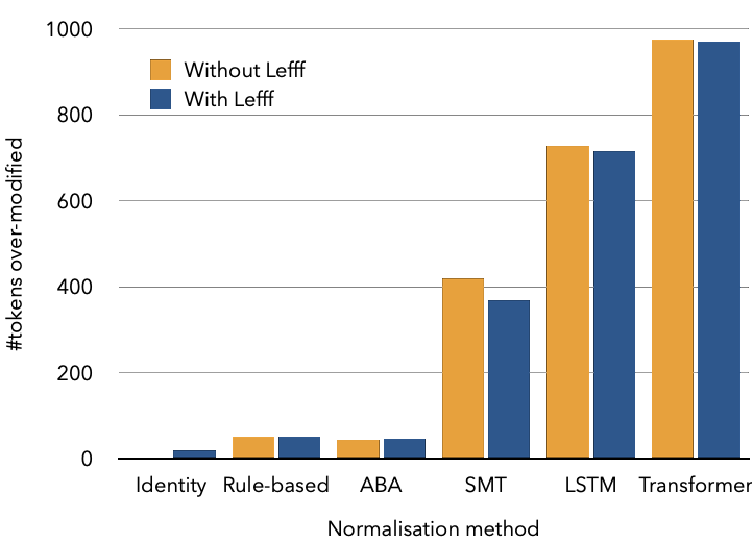
\includegraphics[width=\linewidth]{nlp-for-ch/images/overmodifications.pdf}
                    \caption{Over-modifications}
                    \label{fig:overmodifications}
                \end{figure}
            \end{column}
            \begin{column}{.48\textwidth}
                \begin{figure}
                    \centering
                    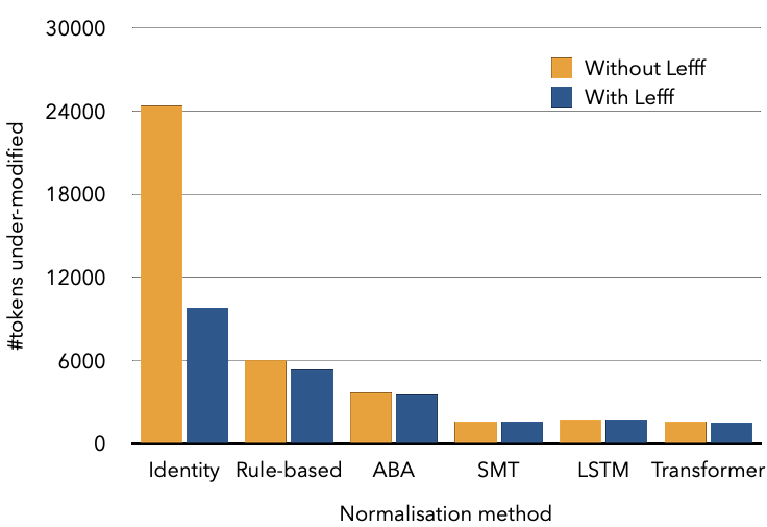
\includegraphics[width=\linewidth]{nlp-for-ch/images/undermodifications.pdf}
                    \caption{Under-modifications}
                    \label{fig:undermodifications}
                \end{figure}
            \end{column}
        \end{columns}
    \end{frame}

%---------------------------------------------------------------

    \section{Beyond ecdotics}

    \begin{frame}
	\begin{center}
            Beyond ecdotics
	\end{center}
    \end{frame}

%---------------------------------------------------------------

    \begin{frame}[fragile]{Output}
        \vspace{2em}
        {It is not only the result of the normalisation that should be preserved, but \textit{all} states of the text.}
        \begin{figure}
        \begin{minted}[tabsize=1, fontsize=\tiny, xleftmargin=5pt, xrightmargin=5pt]{xml}
        <sp>
           <ab>
              <seg>
                 <orig>Promettez-moy donc, Seigneur Geronimo, de me parler avec toute
                 ſorte de franchiſe.</orig>
                 <reg>Promettez-moi donc, Seigneur Geronimo, de me parler avec toute
                 sorte de franchise.</reg>
              </seg>
           </ab>
        </sp>
        <sp>
           <ab>
              <seg>
                 <orig>Ie vous le promets.</orig>
                 <reg>Je vous le promets.</reg>
              </seg>
           </ab>
        </sp>
        \end{minted}
            \caption{Example of TEI encoding with normalisation.}
            \label{fig:tei}
        \end{figure}
    \end{frame}

%---------------------------------------------------------------

    \begin{frame}{Layer-based philology}
    
        Rather than having just one version of the text, we can now have several, which can allow for different uses.
        \begin{itemize}
            \item We can read the semi-diplomatic version of text;
            \item If, rather than producing only a (semi-)diplomatic version of the text, one produces a version fully aligned with the contemporary language, one can use NLP tools unavailable for historical states of a language;
            \item We can search via the contemporary form (\textit{était}) all occurrences despite the graphic variation (\textit{était}, \textit{étoit}, \textit{estoit})…
        \end{itemize}

        The importance of normalisation goes beyond ecdotics!
        
    \end{frame}

%---------------------------------------------------------------

    \begin{frame}{Analysing historical spelling systems}
        \vspace{1.2em}
        By comparing the original source version (horizontal) and the standardized version aligned with the contemporary language (vertical), one can analyse the distance between the two states.
        \begin{figure}
            \centering
            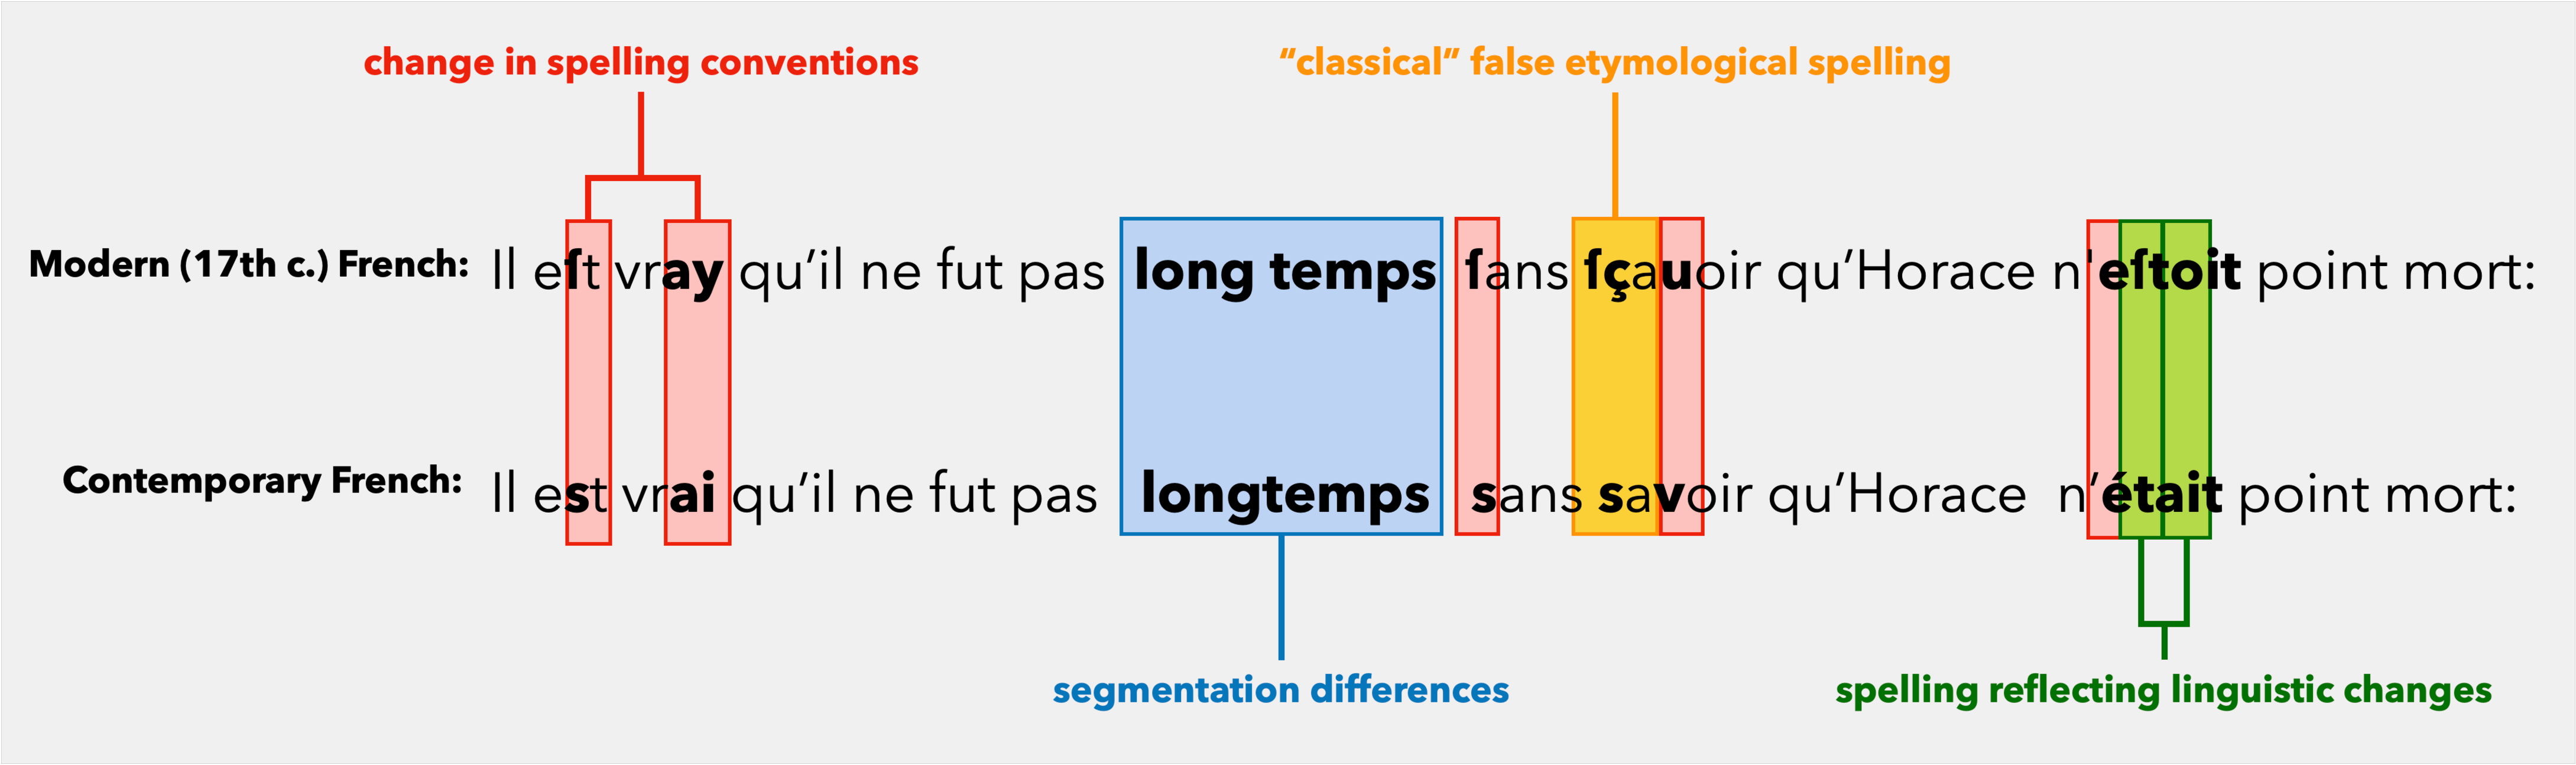
\includegraphics[width=\linewidth]{nlp-for-ch/images/main-example.pdf}
            \caption{Example of different types of changes between 17th c. French and contemporary French.}
            \label{fig:comparison}
        \end{figure}
    \end{frame}

%---------------------------------------------------------------

    \begin{frame}{Study of linguistic change}
        \vspace{1em}
        \begin{figure}
            \centering
            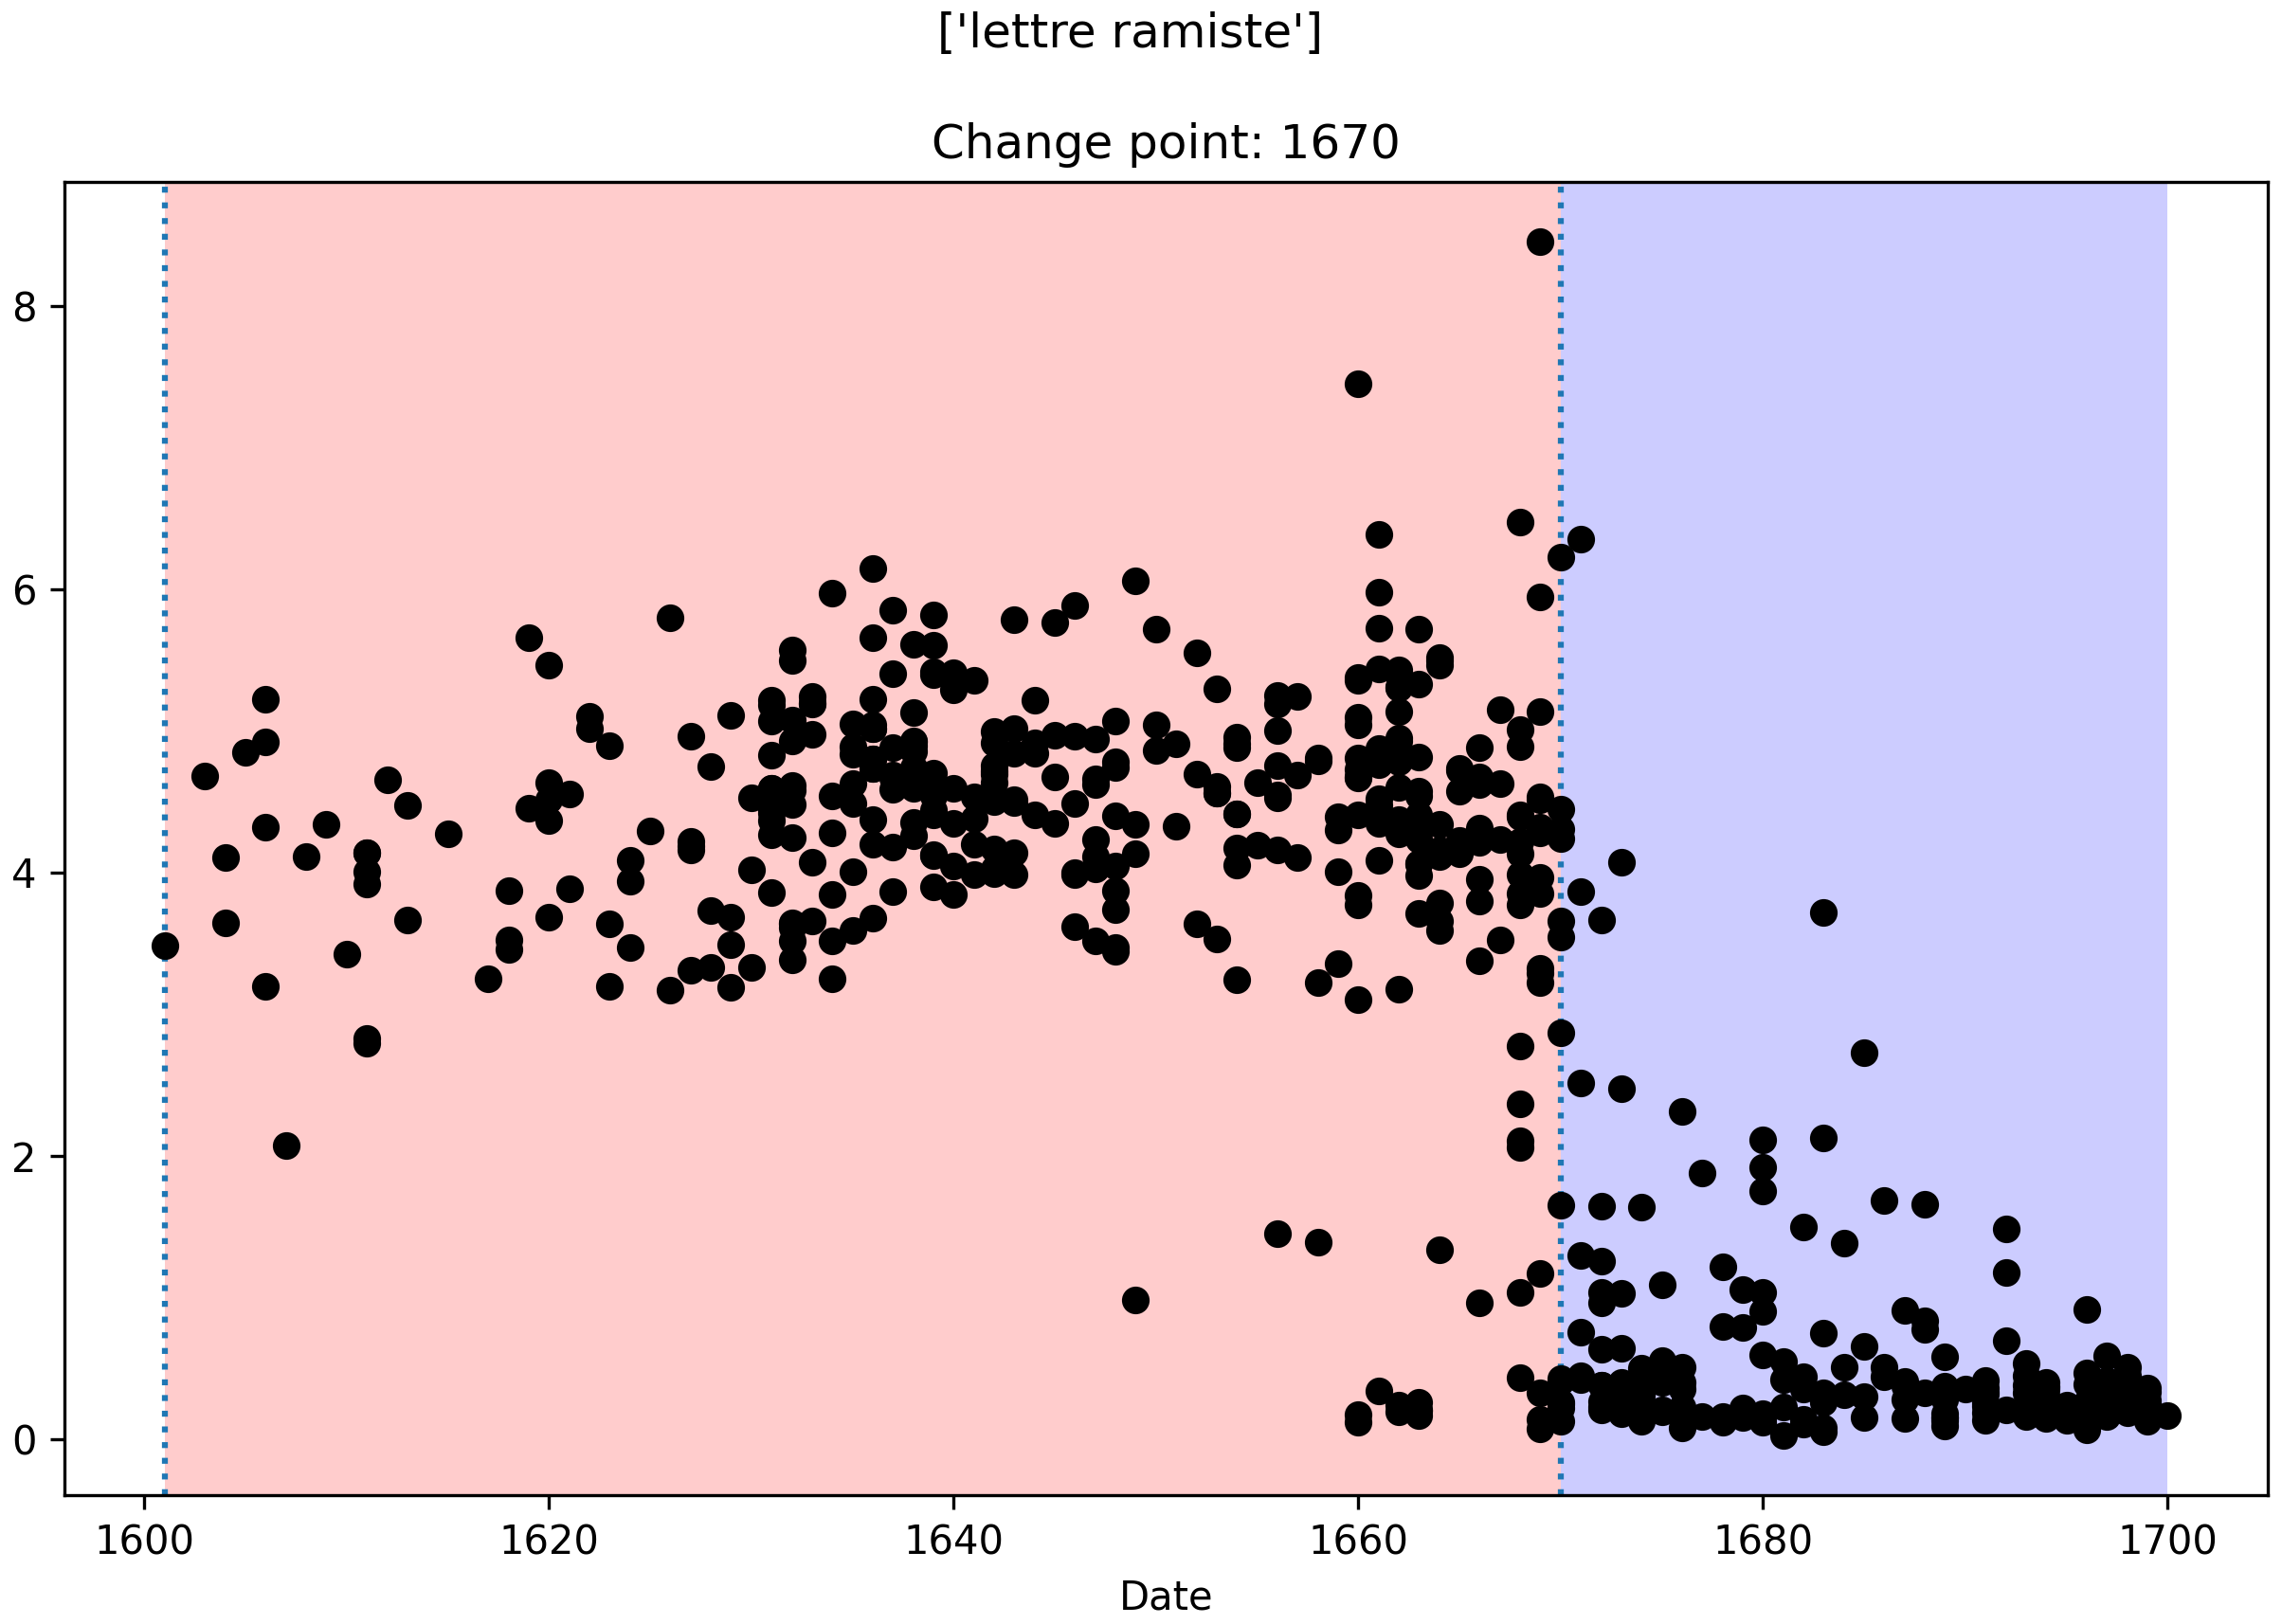
\includegraphics[width=.6\linewidth]{nlp-for-ch/images/3_cptd_ramiste.png}
            \caption{Dating of the introduction of the letters \textit{v} and \textit{j} in French.}
            \label{fig:3_cptd_ramiste}
        \end{figure}
    \end{frame}

%---------------------------------------------------------------

    \begin{frame}{}
        \centering
        Thank you!
    \end{frame}

%---------------------------------------------------------------

\begin{frame}{Selected bibliography}
    \begin{itemize}
        \footnotesize
        \item Simon Gabay, Thibault Clérice. The birth of French orthography. A computational analysis of French spelling systems in diachrony. \textit{CHR2024 – Computational Humanities Research Conference}, Dec. 2024, Aahrus, Denmark. \href{https://inria.hal.science/hal-04704549}{⟨hal-04704549⟩}.
        \item Rachel Bawden, Jonathan Poinhos, Eleni Kogkitsidou, Philippe Gambette, Benoît Sagot, et al.. Automatic Normalisation of Early Modern French. \textit{LREC 2022 - 13th Language Resources and Evaluation Conference}, European Language Resources Association, Jun 2022, Marseille, France. pp.3354-3366. \href{https://inria.hal.science/hal-03540226}{⟨hal-03540226v2⟩}.
        \item Simon Gabay, Loïc Barrault. Traduction automatique pour la normalisation du français du XVIIe siècle. \textit{6e conférence conjointe Journées d'Études sur la Parole (JEP, 33e édition), Traitement Automatique des Langues Naturelles (TALN, 27e édition)}. Volume 2 : Traitement Automatique des Langues Naturelles, 2020, Nancy, France. pp.213-222. \href{https://hal.science/hal-02784770}{⟨hal-02784770v3⟩}.
    \end{itemize}
    
\end{frame}
\end{document}